\clearpage
\makeatletter
\setlength{\@fptop}{0pt}
\makeatother
\begin{figure*}[p!]
  \centering
  \begin{subfigure}[t]{0.24\textwidth}
    \centering
    
\includegraphics[width=\linewidth]{../dataset/figures/fig_042.png}
    \caption{Clean}
  \end{subfigure}
  \hfill
  \begin{subfigure}[t]{0.24\textwidth}
    \centering
    
\includegraphics[width=\linewidth]{../dataset/transforms/noise/fig_042.png}
    \caption{Gaussian noise}
  \end{subfigure}
  \hfill
  \begin{subfigure}[t]{0.24\textwidth}
    \centering
    
\includegraphics[width=\linewidth]{../dataset/transforms/low_contrast/fig_042.png}
    \caption{Low contrast}
  \end{subfigure}
  \hfill
  \begin{subfigure}[t]{0.24\textwidth}
    \centering
    
\includegraphics[width=\linewidth]{../dataset/transforms/rotation/fig_042.png}
    \caption{Rotation}
  \end{subfigure}

  \vspace{0.65em}

  \begin{subfigure}[t]{0.24\textwidth}
    \centering
    
\includegraphics[width=\linewidth]{../dataset/transforms/in_paper/fig_042.png}
    \caption{In paper}
  \end{subfigure}
  \hfill
  \begin{subfigure}[t]{0.24\textwidth}
    \centering
    
\includegraphics[width=\linewidth]{../dataset/transforms/in_paper_blur/fig_042.png}
    \caption{In-paper blur}
  \end{subfigure}
  \hfill
  \begin{subfigure}[t]{0.24\textwidth}
    \centering
    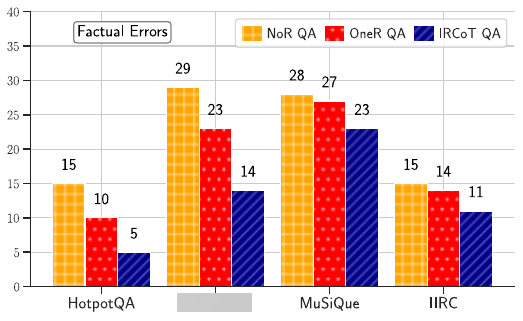
\includegraphics[width=\linewidth]{../dataset/adversarial/admittance/fig_042.png}
    \caption{Admittance blur}
  \end{subfigure}
  \hfill
  \begin{subfigure}[t]{0.24\textwidth}
    \centering
    
\includegraphics[width=\linewidth]{../dataset/adversarial/inductance/fig_042.png}
    \caption{Inductance blur}
  \end{subfigure}

  \caption{Representative visual conditions for Figure~042. The first row shows the clean figure and direct perceptual transformations. The second row shows document-context and selective-blur conditions. Admittance blur removes information intended to be unrecoverable; inductance blur removes information selected to remain inferable from context.}
  \label{fig:appendix-degradation-gallery}
\end{figure*}
\clearpage
